\documentclass{article}
\usepackage{multicol}
\usepackage[utf8]{inputenc}
\usepackage[T1]{fontenc}      
\usepackage[francais]{babel}
\usepackage{graphicx}
\usepackage{circuitikz}
\usepackage[squaren, Gray]{SIunits}
\usepackage{sistyle}
\usepackage[autolanguage]{numprint}
\usepackage{pgfplots}
\usepackage[margin=0.8in]{geometry}

\usepackage{hyperref}
\usepackage{caption}
\usepackage{subcaption}
\usepackage{amsmath,amssymb,array}
\usepackage{url}
\usepackage{fancyhdr}
\usepackage{layout}
\usepackage[version=3]{mhchem}
\usepackage{array} 
\usepackage{tikz}
	\usetikzlibrary{arrows,shapes,positioning}


\newcommand{\reporttitle}{Analyse dynamique}     % Titre
\newcommand{\reportauthor}{Geoffroy \bsc{Jacquet} \\ Corentin \bsc{Joachim}\\ Léa \bsc{Paulus}} % Auteur
\newcommand{\reportsubject}{Rapport de projet en construction mécanique 1} % Sujet
\newcommand{\HRule}{\rule{\linewidth}{0.5mm}}
\newcommand{\copyrigh}{{\tiny \textregistered}}
\setlength{\parskip}{1ex} % Espace entre les paragraphes

\hypersetup{
    pdftitle={\reporttitle},%
     pdfauthor={\reportauthor},%
    pdfsubject={\reportsubject},%
    pdfkeywords={rapport} {vos} {mots} {clés}
}


\setlength{\headheight}{12pt}
\setlength{\headsep}{12pt}

\pagestyle{fancy}
\lhead{\leftmark{}}
\rhead{LMECA1210 - 2015 - gr11}
\cfoot{\thepage{}}
\begin{document}
\begin{titlepage}

\begin{center}

% Upper part of the page

\textsc{\Large Université Catholique de Louvain}\\[0.5cm]

\textsc{\LARGE Rapport de projet en construction mécanique 1}\\[0.2cm]
\textsc{\LARGE LMECA1210}\\[0.2cm]

% Title
\HRule \\[0.2cm]
{\huge \bfseries Analyse dynamique}\\
\HRule \\[0.2cm]

% Author and supervisor
\begin{center}
\includegraphics[trim=0cm 8cm 0cm 5cm, clip, width= 15 cm, height= 13 cm ]{Schema/bielle2.jpg}
\end{center}
\HRule \\[0 cm]


\begin{minipage}{0.4\textwidth}
\begin{flushleft} \large

\begin{tabular}{l l}

\emph{Auteurs:} & \\
 
Geoffroy & \bsc{Jacquet}\\ 
Corentin & \bsc{Joachim}\\ 
Léa & \bsc{Paulus}

\end{tabular}
\end{flushleft}
\end{minipage}
\begin{minipage}{0.4\textwidth}
\begin{flushright} \large
\emph{Cours:} \\
LMECA1210\\
\emph{Groupe:} \\
11\\
\emph{Professeur:} \\
Hervé \textsc{Jeanmart}
\end{flushright}
\end{minipage}
\vspace{0.6cm}
% Bottom of the page

\begin{minipage}{0.3\textwidth}
\begin{flushleft}
\includegraphics[height=2cm]{Schema/logo_UCL_NEW_janv2013.JPG}
\end{flushleft}
\end{minipage}
\begin{minipage}{0.3\textwidth}
\begin{center}
{\large FSA12BA}\\
{\large \today}
\end{center}
\end{minipage}
\begin{minipage}{0.3\textwidth}
\begin{flushright}
\includegraphics[height=1cm]{Schema/epl-logo.jpg}
\end{flushright}
\end{minipage}
\end{center}
\end{titlepage}
%\tableofcontents



\section{Détermination des grandeurs géométriques du moteur}

\begin{center}
\begin{tabular}{|c|c|c|c|}
\hline 
\textbf{Grandeur} & \textbf{Symbole} & \textbf{Valeur} & \textbf{Unités} \\ 
\hline 
Diamètre piston & $D$ & 0.075 & \meter \\ 
\hline 
Longueur manivelle & $R$ & 0.03675 & \meter \\ 
\hline 
Longueur bielle & $L$ & 0.12885 & \meter \\ 
\hline 
Cylindrée & $V_c$ & 324.25 & \cubic\centi\metre \\ 
\hline 
Taux de compression & $\tau$ & 8.2 & / \\ 
\hline 
\end{tabular} 
\end{center}

Pour trouver le taux de compression de notre moteur, nous nous sommes basé sur les données issues d'iCampus~\cite{icampus} pour trouver le moteur correspondant. Il s'agit d'un moteur GM provenant d'une Opel Kadett de 1979 ou 1985  dont les données ci-dessus sont identiques et le taux de compression est de \unit{8.2} (voir~\cite{carspector} et~\cite{carfolio}).


Concernant les groupes partenaires, nous n'en n'avons pas, nous étions à une table sans autres groupes, la table 14.

\section{Évolution de le pression dans le cylindre}
Le graphique que nous avons obtenu sur Matlab se trouve à la figure~\ref{fig:pression}.
\begin{figure}{h!}
\centering
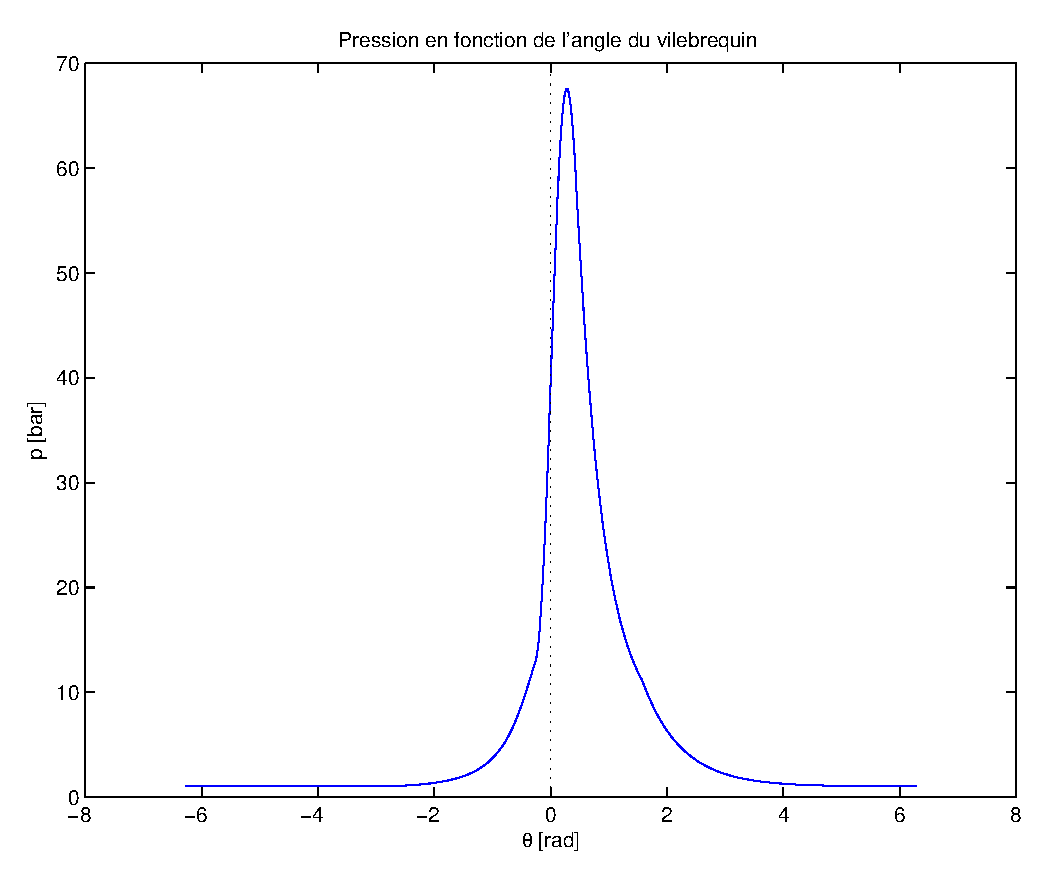
\includegraphics[scale=0.65]{Schema/pression.eps}
\caption{Évolution de la pression dans le cylindre}
\label{fig:pression}
\end{figure}


\section{Efforts sur la bielle}

Les deux courbes à la figure~\ref{fig:EffortBielle} représentent ici respectivement les efforts sur le pied et la tête de la bielle. Puisque les deux forces sont représentées positives vers le bas, il s'agit de compression lorsque la force sur le pied est positive, et celle sur la tête négative, et de traction dans l'autre cas. 

\begin{figure}[h]
%\centering
    \begin{subfigure}[h]{0.45\textwidth}
    				\includegraphics[scale=0.5]{Schema/forces_3000rpm.eps}
                \caption{\unit{3000}{rpm}}
                \label{fig:forces_3000rpm}
    \end{subfigure}
    \qquad
    \begin{subfigure}[h]{0.45\textwidth}
        			\includegraphics[scale=0.5]{Schema/forces_5000rpm.eps}
                \caption{\unit{5000}{rpm}}
                \label{fig:forces_5000rpm}
    \end{subfigure}
    \caption{Efforts sur la bielle}
    \label{fig:EffortBielle}
\end{figure}


Les tableaux~\ref{fig:EffortMaxtrac} reprennent les efforts maximums de traction et de compression :

\begin{figure}[h]
\centering
    \begin{subfigure}[h]{0.45\textwidth}
    		\begin{tabular}{|c|c|c|}
		\hline 
  		& \textbf{Pied} & \textbf{Tête} \\ 
		\hline 
		\textbf{Compression} & \unit{28.786}{ \kilo\newton} & \unit{26.887}{\kilo\newton} \\ 
		\hline 
		\textbf{Traction} & \unit{0.677}{ \kilo\newton} & \unit{2.650}{ \kilo\newton} \\ 
		\hline 
		\end{tabular}
		\caption{\unit{3000}{rpm}}
		\label{fig:tab_forces_3000rpm}
    \end{subfigure}
    \begin{subfigure}[h]{0.45\textwidth}
        	\begin{tabular}{|c|c|c|}
		\hline 
  		& \textbf{Pied} & \textbf{Tête} \\ 
		\hline 
		\textbf{Compression} & \unit{26.862}{ \kilo\newton} & \unit{21.601}{ \kilo\newton}\\ 
		\hline 
		\textbf{Traction} & \unit{2.676}{ \kilo\newton} & \unit{8.157}{\kilo\newton} \\ 
		\hline 
		\end{tabular} 	
		\caption{\unit{5000}{rpm}}
		\label{fig:tab_forces_5000rpm}	
    \end{subfigure}
    \caption{Efforts maximums de traction et de compression}
    \label{fig:EffortMaxtrac}
\end{figure}

Afin de représenter l'effort total que subit la bielle, il faut donc faire la différence de l'effort sur le pied avec celui sur la tête.

La partie positive des graphes de la figure~\ref{fig:Effort_totaux} représente un effort de compression tandis que le négative représente de la traction.

\begin{figure}[h!]
%\centering
    \begin{subfigure}[h!]{0.45\textwidth}
    				\includegraphics[scale=0.5]{Schema/forces_tot_3000rpm.eps}
                \caption{\unit{3000}{rpm}}
                \label{fig:forces_tot_3000rpm}
    \end{subfigure}
    \qquad
    \begin{subfigure}[h!]{0.45\textwidth}
                \includegraphics[scale=0.5]{Schema/forces_tot_5000rpm.eps}
                \caption{\unit{5000}{rpm}}
                \label{fig:forces_tot_5000rpm}
    \end{subfigure}
    \caption{Effort totaux subits par la bielle}
    \label{fig:Effort_totaux}
\end{figure}

Les efforts maximums et minimums sont repris dans les tableaux~\ref{fig:max_3000rpm} et~\ref{fig:max_5000rpm}. Les efforts minimums sont 0; il est logique que lorsqu'il y a de la traction, il n'y ait pas de compression et vice-versa.


\begin{figure}[h!]
\centering
    \begin{subfigure}[h]{0.45\textwidth}
    		\begin{tabular}{|c|c|c|}
    		\hline
    		&\textbf{Max}&\textbf{Min}\\
		\hline 
		\textbf{Compression} & \unit{55.670}{\kilo\newton} & 0\\ 
		\hline 
		\textbf{Traction} & \unit{3.327}{\kilo\newton} & 0\\ 
		\hline 
		\end{tabular} 
        \caption{\unit{3000}{rpm}}
        \label{fig:max_3000rpm}
    \end{subfigure}
    \begin{subfigure}[h]{0.45\textwidth}
        \begin{tabular}{|c|c|c|}
        \hline
    		&\textbf{Max}&\textbf{Min}\\
		\hline 
		\textbf{Compression} & \unit{48.462}{\kilo\newton}&0 \\ 
		\hline 
		\textbf{Traction} & \unit{10.832}{\kilo\newton} &0\\ 
		\hline 
		\end{tabular} 
        \caption{\unit{5000}{rpm}}
        \label{fig:max_5000rpm}
    \end{subfigure}
    \caption{}
\end{figure}



\section{Justification de la forme en "I"}
La bielle étant contrainte à des efforts de traction et principalement de compression, pour un fonctionnement optimal dans un moteur à haute vitesse il faut que celle-ci soit à la fois élancée, légère tout en étant capable de résister aux sollicitations. La forme qui répond le mieux à l'ensemble de ces critères s'avère être la forme en I.



\section{Dimensionnement de la section de la bielle}

Nous avons effectué divers calculs afin de dimensionner la section (effort de flambage) nécessaire pour que la bielle résiste aux différents efforts calculés précédemment. Pour cela, nous avons utilisé la formule de Rankine, à savoir : 
{$$\sigma_{fb Rankine} = \frac{F_b}{A_{crit}}(1+\lambda^2) = \frac{R_e}{S_{Rankine}}$$
En sachant que : 
$$ \lambda = \frac{\lambda_{barre}}{\lambda_{lim Euler}}, $$
$$ \lambda_{barre} = \frac{l_{f}}{I_g},$$
$$ i_g = \sqrt{\frac{I}{A_{crit}}},$$ 
et
$$ \lambda_{lim Euler} = \pi \sqrt{\frac{E}{R_e}}.$$
\begin{center}
 \begin{tabular}{|c|c|c|}

        \hline
    		\textbf{Notations}&\textbf{Significations}&\textbf{Valeurs}\\
		\hline 
		$\sigma_{fb Rankine}$ & Contrainte de flambement suivant Rankine & \unit{241,18}{} \\ 
		\hline 
		$R_e$ & Limite d'élasticité & \unit{410}{\pascal} \\ 
		\hline 
		$E$ & Module de Young & \unit{170000}{\pascal} \\ 
		\hline 
		$\lambda_{lim Euler}$ & L'élancement limite d'Euler & $ \lambda_{lim Euler} = \pi \sqrt{\frac{E}{R_e}}$ \\ 
		\hline 
		$\lambda_{barre}$ & Élancement réel de la barre & $ \lambda_{barre} = \frac{l_{f}}{I_g}$\\
		\hline 
		$i_g$ & Rayon de giration de la section critique & $ i_g = \sqrt{\frac{I}{A_{crit}}}$ \\
		\hline 
		$\lambda$ & L'élancement réduit & $ \lambda = \frac{\lambda_{barre}}{\lambda_{lim Euler}} $ \\
		\hline 
		$F_b$ & Effort total maximum transmis par la bielle & \unit{4,8\cdot 10^4}{Newton}\\
		\hline 
		$l_f$ & Longueur de flambement & \unit{0.1285}{} \\
		\hline 
		$S_{Rankine}$ & Coefficient de sécurité & {1,7} [/] \\
		\hline 
		$I$ & Moment d'inertie de la section & \unit{3489,84}{\pascal} \\
		\hline
		$A_{crit}$ & Section critique & Inconnue\\
		\hline 
\end{tabular}
\end{center}		
Remarque pour le calcul du moment d'inertie de la section: en se référant à la figure (LEAAAA) pour les différentes longueurs de la section en "I". Sur base de celle-ci, le moment d'inertie vaut:
$$ I = \frac{1}{12} (2,25t (3,4t)^3 - 2,3t (2,3t)^3) = \unit{5,86}{mm^2}$$
Maintenant que toutes les valeurs sont connues, il ne nous reste plus qu'à isoler notre inconnue, à savoir la section, puis de résoudre grâce à Matlab. A savoir : 

$$ A_{crit} = - \frac{F_b}{\sigma ( \frac{F_B (l_f)^2}{\sigma \lambda_l I} - 1)} = \unit{1,99}{cm^2}$$

Nous pouvons donc comparer la valeur théorique obtenue ci-dessus avec la section réelle de notre bielle mesurée en laboratoire. Cette section est approximativement de 
\unit{147,19}{mm^2} à laquelle il faut encore ajouter l'aire occupée par les partie arrondie de la section. On peut donc conclure que la valeur théorique obtenue est sensiblement proche de la valeur réelle.
		

\begin{thebibliography}{9}

\bibitem{carspector}
\url{http://carspector.com/car/opel/009029/}

\bibitem{icampus}
\url{http://icampus.uclouvain.be/claroline/backends/download.php?url=L01lc3VyZXNfZXRfcGxhbnMvTE1FQ0ExMjEwXy1fTGlzdGVfZGVzX21vdGV1cnNfMjAxNS5wZGY%3D&cidReset=true&cidReq=LMECA1210}

\bibitem{carfolio}
\url{http://www.carfolio.com/specifications/models/car/?car=11319}
\end{thebibliography}

%\bibliography{biblio}{}
%\bibliographystyle{plain}
\end{document}